\section{Hardware accelerators}

The rise and extensive adoption of Deep Learning models have ushered in a new era where specialized hardware is essential for powering various machine learning (ML) solutions.
Since 2013, the computational demands for AI training have doubled approximately every four months, significantly outpacing the traditional Moore's Law projection of two years.
To meet the increasing computational requirements of Deep Learning tasks, WSC are now deploying specialized accelerator hardware optimized for the intensive processing needed for training and inference tasks in Deep Learning applications.

\subsection{Graphical Processing Unit}
Graphical Processing Unit (GPU) have transformed data processing by enabling data-parallel computations, where the same program can be executed simultaneously on multiple data elements. 
This parallelization is particularly effective for scientific codes, which often revolve around matrix operations.
Using high-level languages, GPUs offer significant speed improvements over traditional CPU-based processing.

\subsection{Neural Networks}
Neural Networks (NN) , inspired by the human brain, consist of interconnected nodes or neurons arranged in layers to process and analyze data. 
They learn data representation, enabling them to function as classifiers or regressors. 
The resurgence of interest in NN is attributed to increased data availability and computational power.

In natural neurons, information is transmitted through chemical mechanisms. 
Dendrites gather charges from synapses, which can be either inhibitory or excitatory. 
Once a threshold is reached, the accumulated charge is released, causing the neuron to fire. 
Similarly, an artificial neuron receives input signals, which are weighted and summed. 
This sum undergoes an activation function, determining the neuron's output:
\[h_j(\mathbf{x}\mid \mathbf{w},b)=h_j\left(\sum_{i=1}^{I}w_j x_i-b\right)=h_j\left( \sum_{i=0}^{I}w_i x_i \right)=h_j\left(\mathbf{w}^T \mathbf{x}\right)\]
\begin{figure}[H]
    \centering
    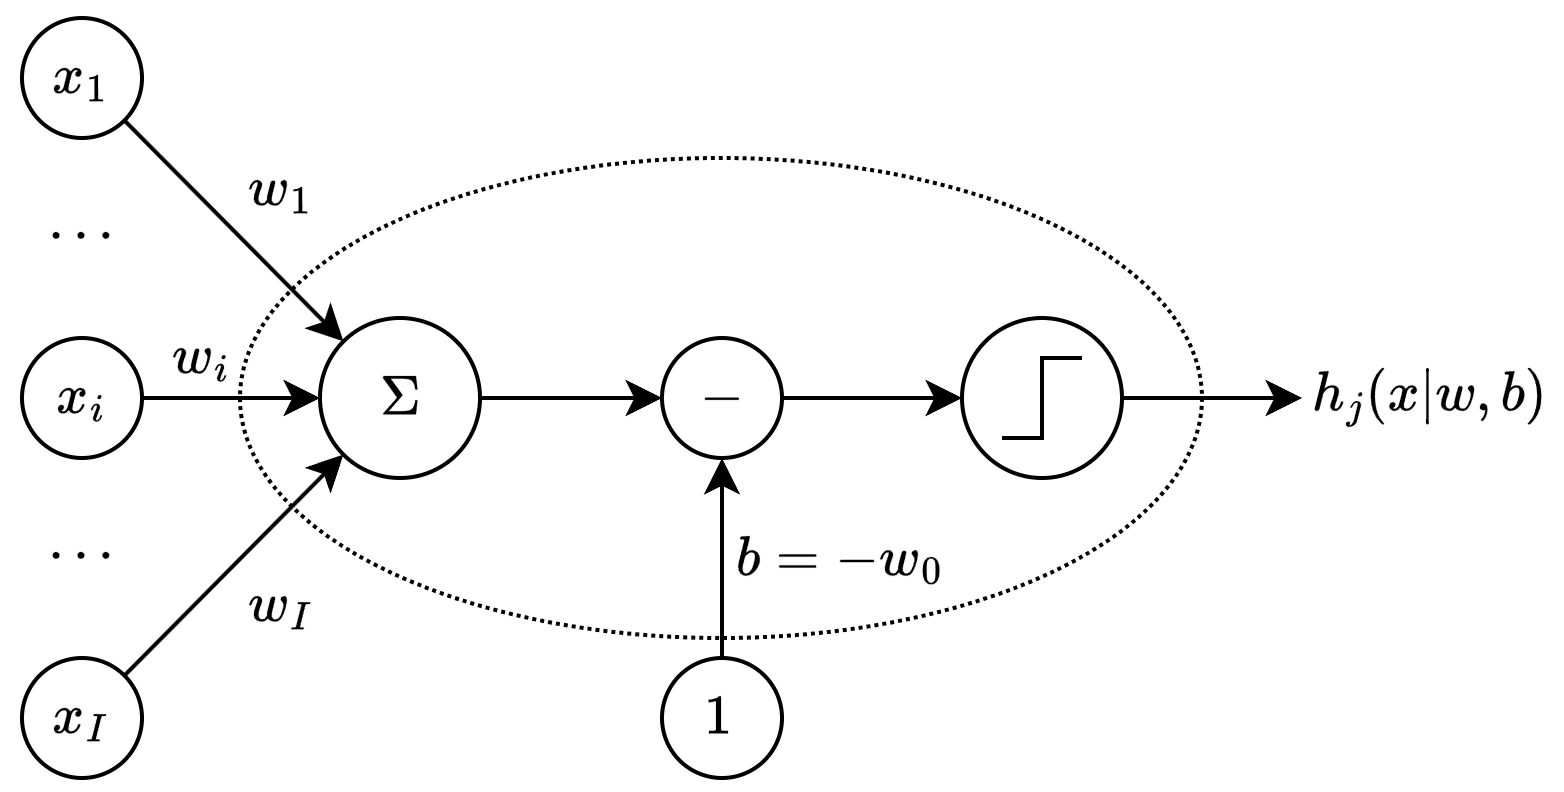
\includegraphics[width=0.5\linewidth]{images/neuron.png}
    \caption{Artificial neuron}
\end{figure}
NN are structured into three main layers:
\begin{itemize}
    \item The input layer, where data is introduced.
    \item The hidden layers, which process and transform the input data.
    \item The output layer, which provides the final results or predictions.
\end{itemize}
These layers are connected through weighted connections and activation functions, which determine the output of each neuron. 
Importantly, the output is influenced solely by the preceding layer's inputs.

NN are inherently non-linear models. 
Their behavior is shaped by various factors, including the number of neurons, the choice of activation functions, and the specific values of the weights.
These factors collectively determine the network's ability to learn and make accurate predictions.

NN learn from historical data during training, often involving back propagation techniques like gradient descent to calculate errors and adjust the model. 
Errors are evaluated and used to refine the network's parameters, improving its prediction or classification accuracy.
Various types of NN are tailored for specific tasks, including:
\begin{itemize}
    \item \textit{Feed Forward NN} (FFNN): where information flows in one direction from input to output.
    \item \textit{Convolutional NN} (CNN): designed for processing grid-like data, such as images, with specialized layers for feature extraction.
    \item \textit{Recurrent NN} (RNN): suitable for sequential data, where past information influences the present, often used in natural language processing and time series analysis.
\end{itemize}
These networks are applied in diverse domains such as image recognition (e.g., facial recognition, object detection) and natural language processing (e.g., chat bots, sentiment analysis).

GPUs are commonly used for training NN. 
However, the performance of such systems is constrained by the slowest learner and the slowest messages transmitted through the network, making a high-performance network essential. 
Typically, a CPU host is connected to a PCIe-attached accelerator tray housing multiple GPUs, which are interconnected using high-bandwidth interfaces like NVlink.
\begin{figure}[H]
    \centering
    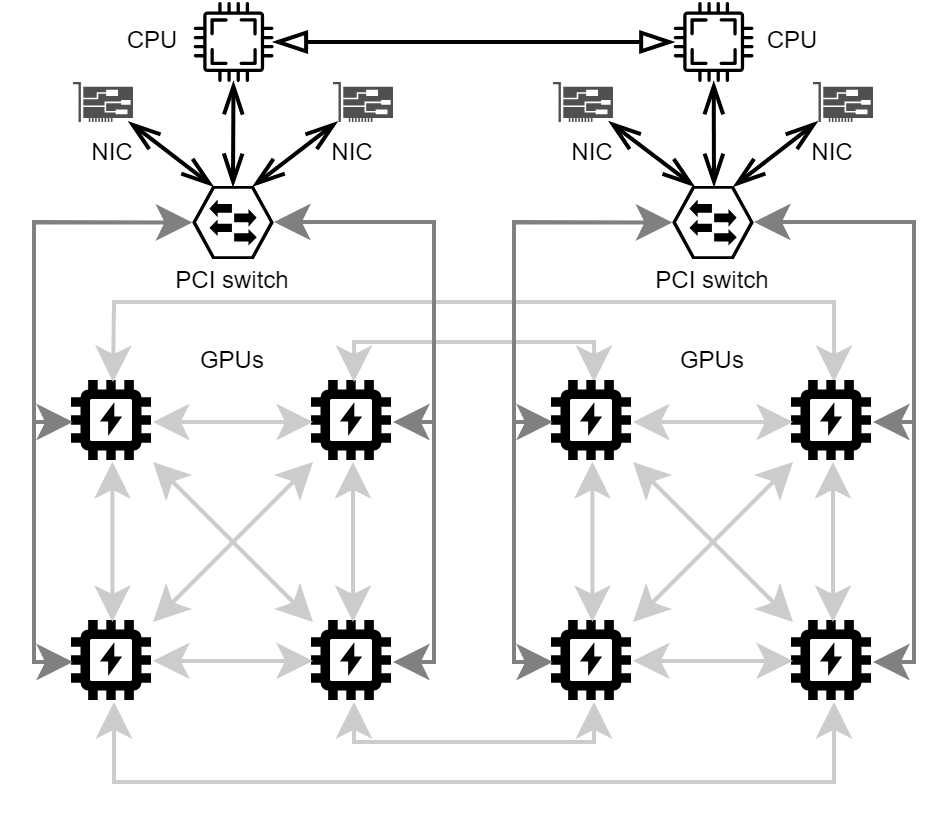
\includegraphics[width=0.75\linewidth]{images/nnt.png}
    \caption{NN training}
\end{figure}

\subsection{Tensor Processing Unit}
Although GPUs are well-suited for ML, they are still considered relatively general-purpose devices. 
Recently, designers have specialized them into ML-specific hardware units, such as Tensor Processing Units (TPU), which have been powering Google data centers since 2015 alongside CPUs and GPUs. 
In TensorFlow, the basic unit of operation is a Tensor, an $n$-dimensional matrix.

TPUs are extensively used for both training and inference tasks, with the main versions being:
\begin{itemize}
    \item \textit{TPUv1}: inference-focused accelerator connected to the host CPU via PCIe links.
    \item \textit{TPUv2}: supports both training and inference, providing enhanced flexibility and performance. 
        Each TPU core consists of an array for matrix computations (MXU) and a connection to high-bandwidth memory (HBM).
    \item \textit{TPUv3}: offers a 2.5 times performance boost compared to TPUv2.
    \item \textit{TPUv4}: delivers a performance increase of approximately 2.7 times compared to TPUv3.
    \item \textit{TPUv5}: an train large language models 2.8 times faster than TPUv4.
\end{itemize}

\subsection{Field Programmable Gate Array}
Field Programmable Gate Arrays (FPGA) are arrays of logic gates that users can program or configure in the field without relying on the original designers. 
These devices consist of carefully designed and interconnected digital sub-circuits that efficiently implement common functions, offering high levels of flexibility. 
The individual sub-circuits within FPGAs are known as Configurable Logic Blocks (CLBs).
Hardware description languages like VHDL and Verilog describe hardware, enabling users to create textual representations of hardware components and their interconnections, similar to a schematic.

\subsection{Summary}
\begin{table}[H]
    \centering
    \begin{tabular}{c|cc}
                  & \textbf{Advantages}                                                                 & \textbf{Disadvantages}                                \\ \hline
    \textit{CPU}  & \makecell{Easily programmable and compatible \\ Rapid design space  \\ Efficiency}  & \makecell{Simple models \\ Small training sets}       \\ \hline
    \textit{GPU}  & \makecell{Parallel execution}                                                       & \makecell{Limited flexibility}                        \\ \hline
    \textit{TPU}  & \makecell{Fast for ML}                                                              & \makecell{Limited flexibility}                        \\ \hline
    \textit{FPGA} & \makecell{High performance \\ Low cost \\ Low power consumption}                    & \makecell{Limited flexibility \\ High-level synthesis}                      
    \end{tabular}
\end{table}